% ══════════════════════════════════════════════════════════════════════
% FIGURES
% ══════════════════════════════════════════════════════════════════════

\begin{figure}[htbp]
\centering
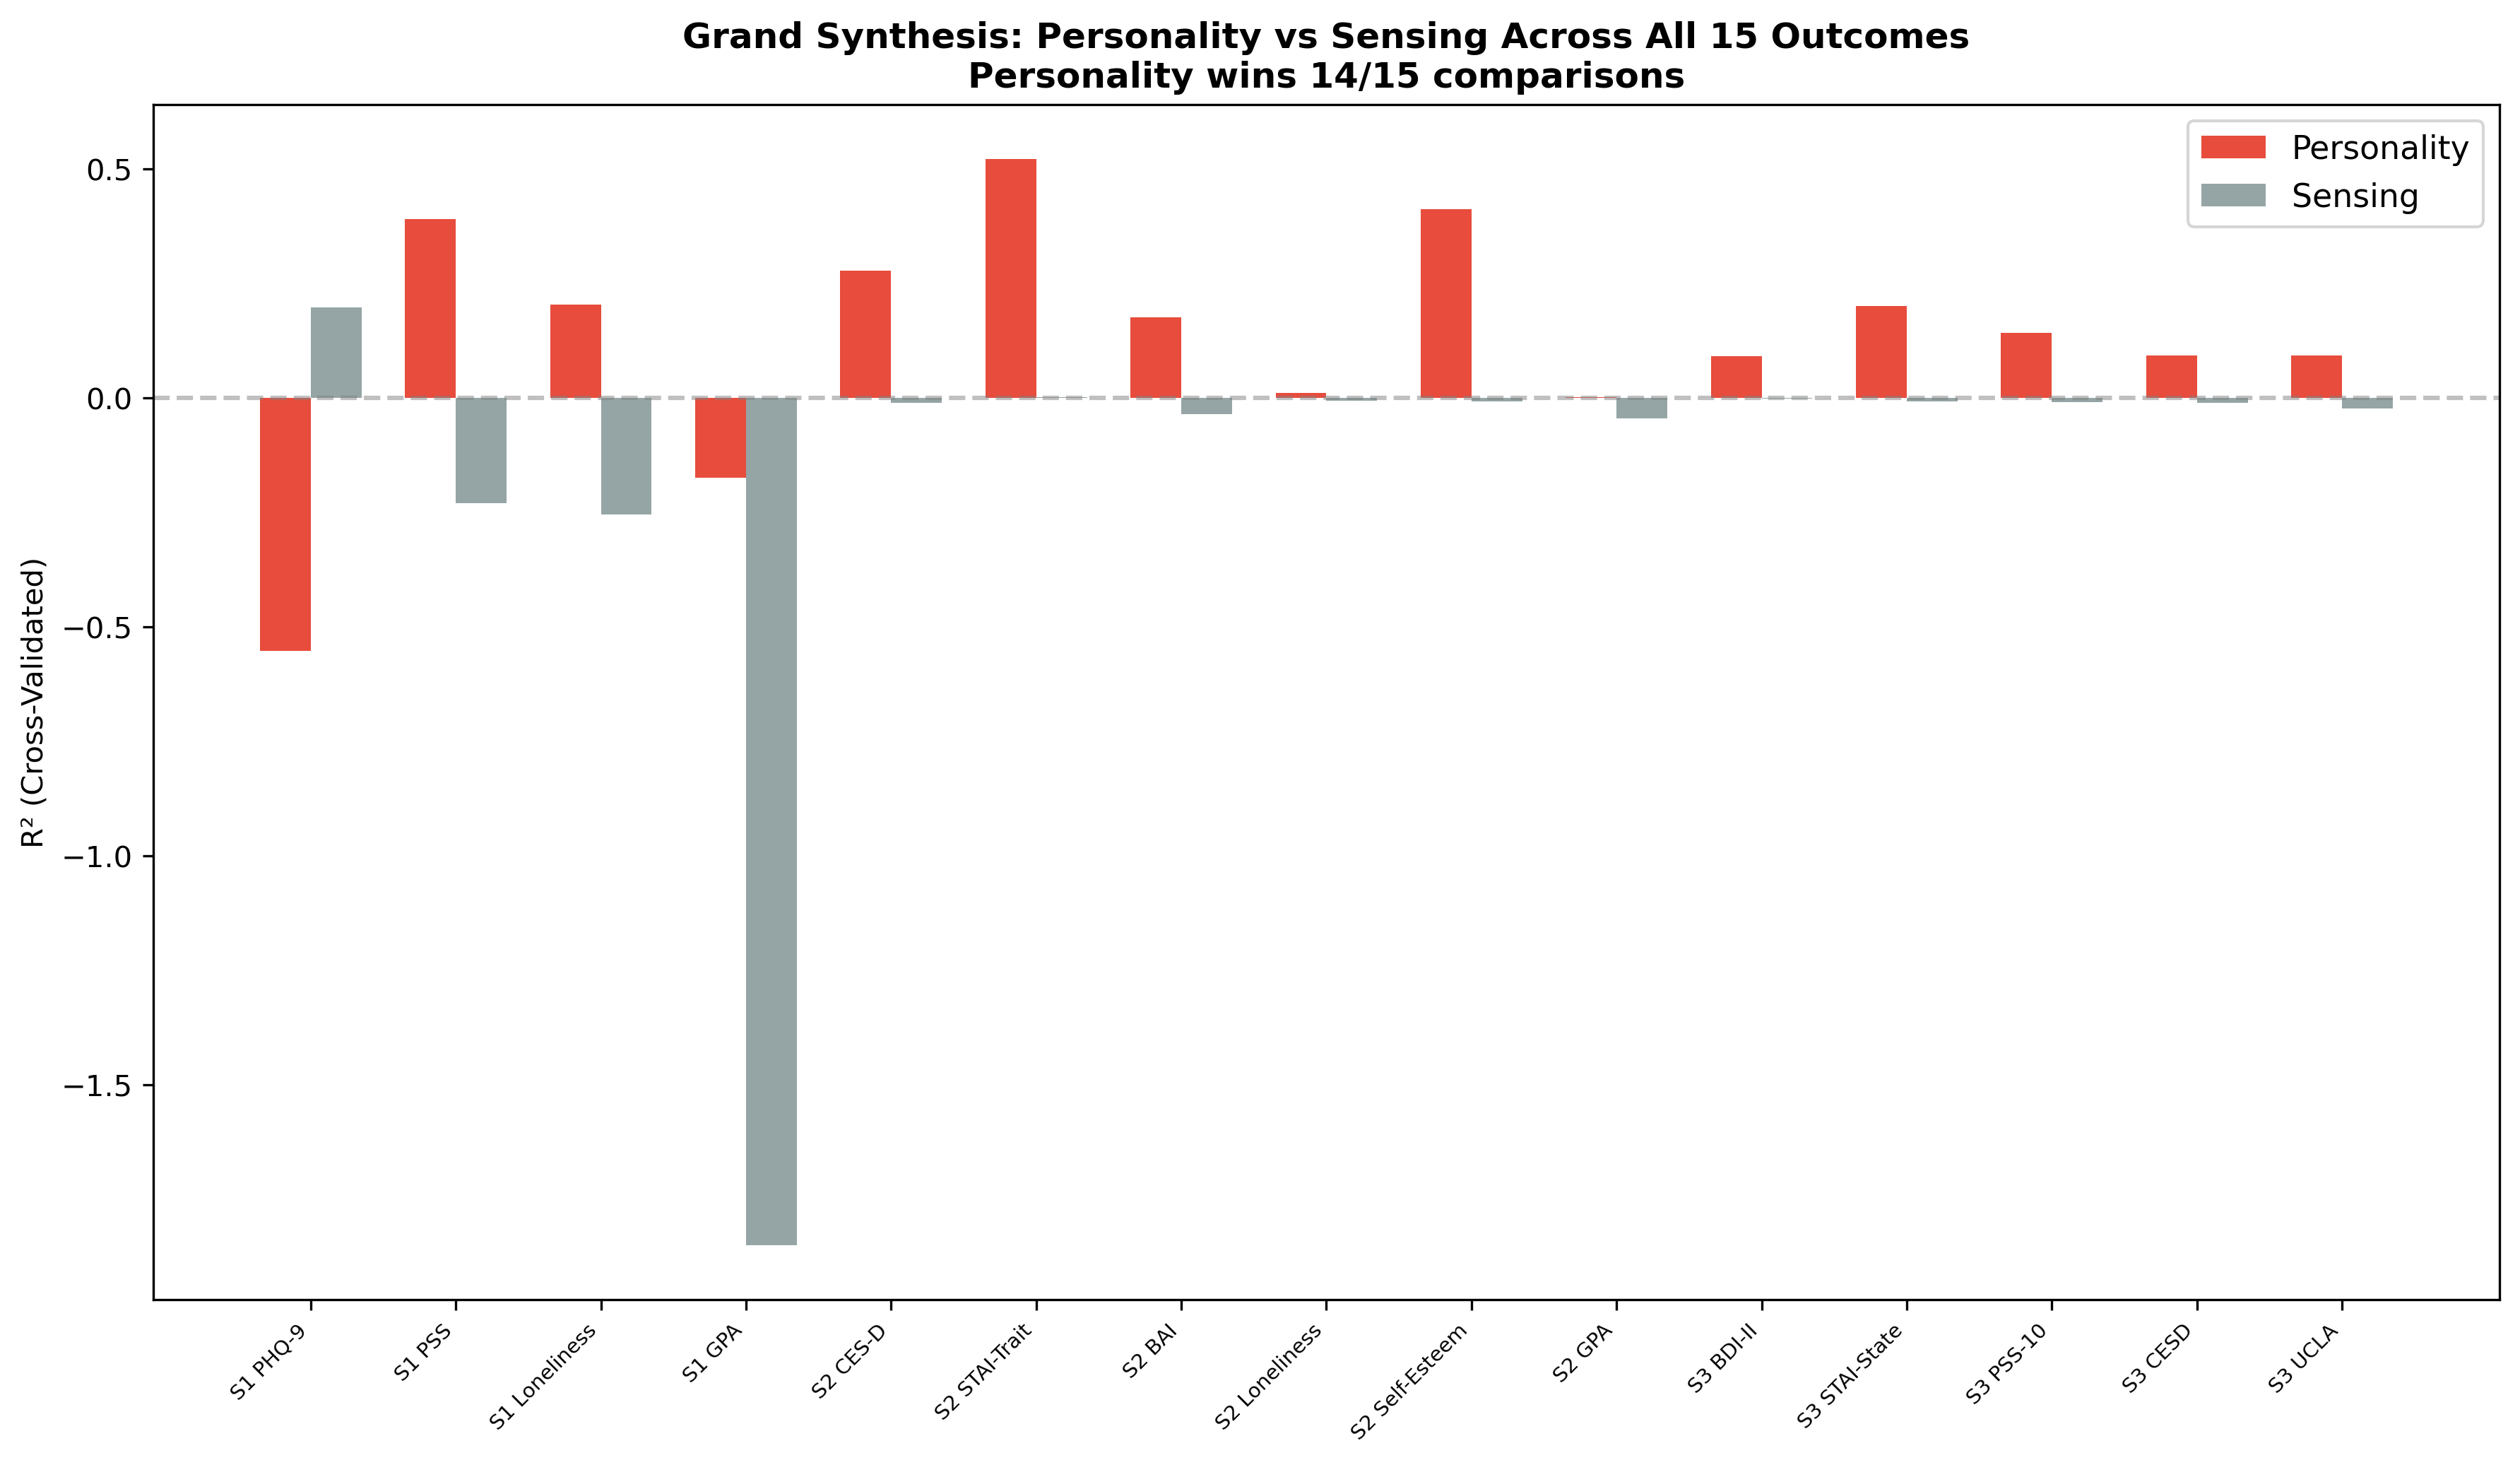
\includegraphics[width=\textwidth]{../results/comparison/supplementary/figure_grand_synthesis.png}
\caption{Grand synthesis of personality versus sensing prediction across three studies and 15 outcomes. Each row represents one study--outcome combination. Personality $R^2$ (blue) and sensing $R^2$ (red) are shown with 95\% confidence intervals from repeated cross-validation. Personality outperformed sensing in 14 of 15 comparisons (93\%). Negative $R^2$ values indicate prediction worse than the intercept-only baseline.}
\label{fig:grand_synthesis}
\end{figure}

\begin{figure}[htbp]
\centering
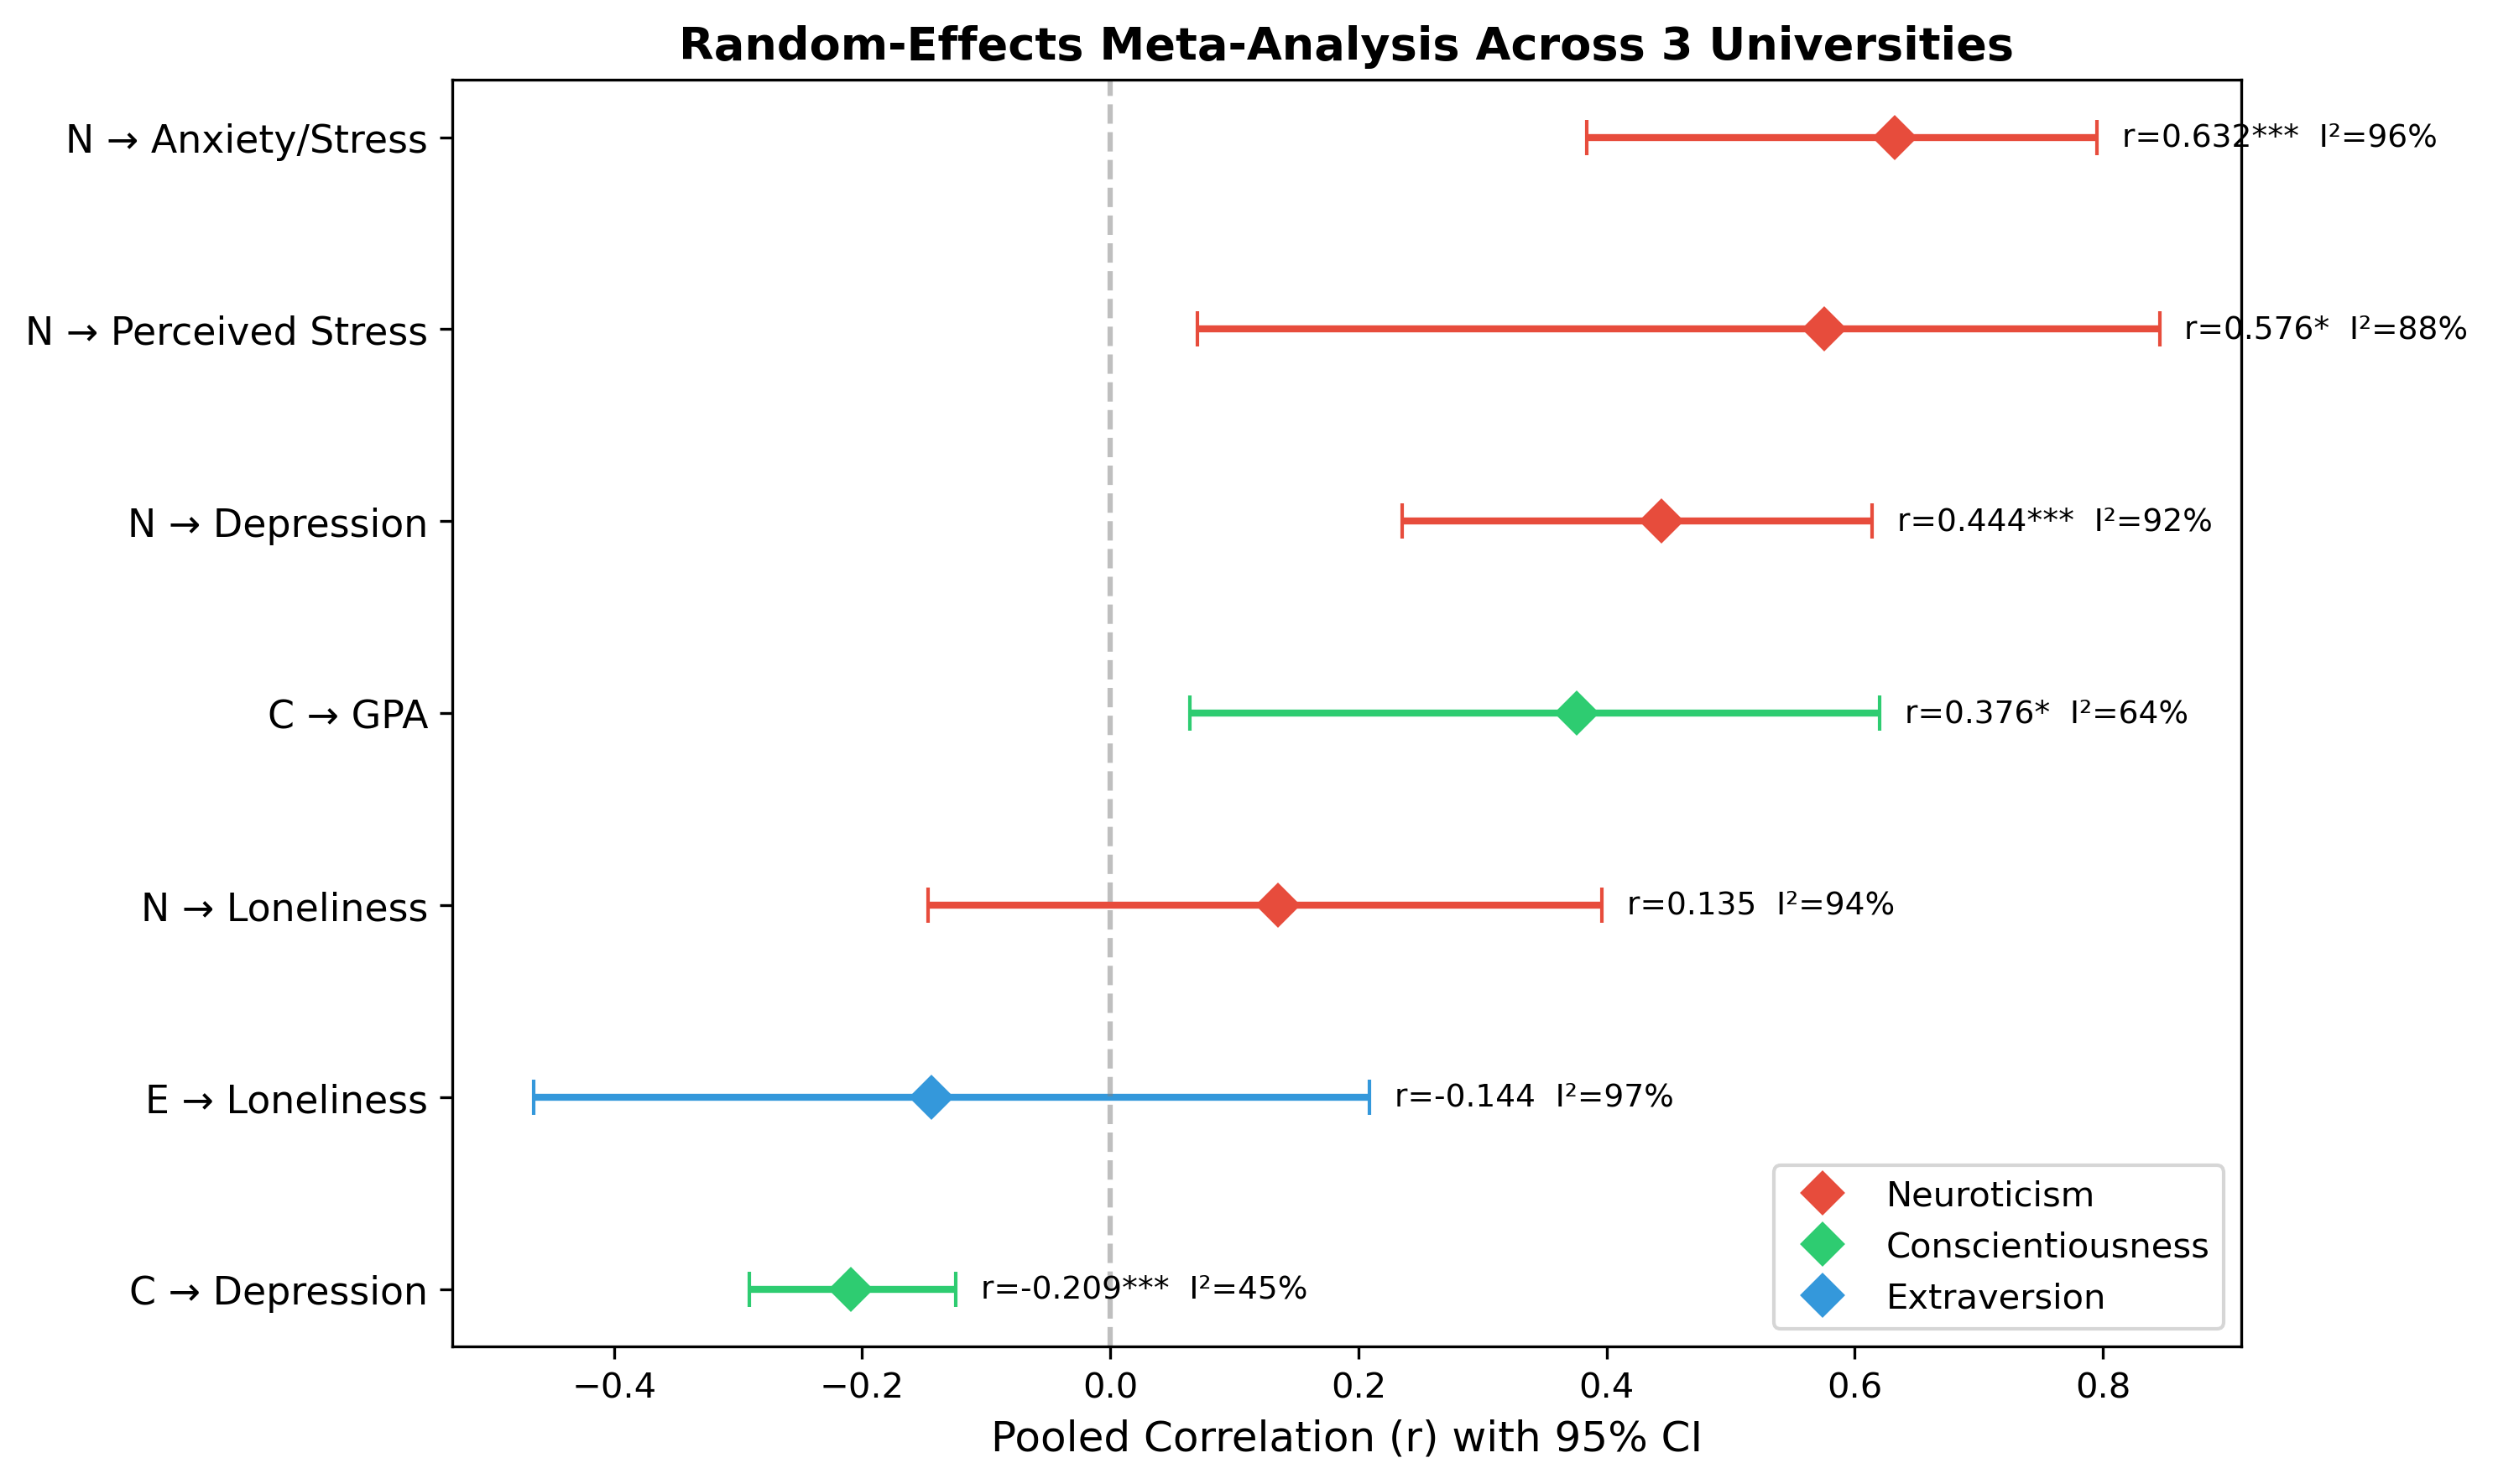
\includegraphics[width=\textwidth]{../results/comparison/meta_analysis_forest.png}
\caption{Forest plots of random-effects meta-analytic estimates for personality--outcome associations across three studies. Effect sizes are Fisher $z$-transformed correlations with 95\% confidence intervals. The strongest and most consistent effects were for Neuroticism predicting depression ($r = .44$) and anxiety/stress ($r = .63$). Diamond indicates the pooled estimate. $I^2$ values indicate the proportion of variability due to between-study heterogeneity.}
\label{fig:forest}
\end{figure}

\begin{figure}[htbp]
\centering
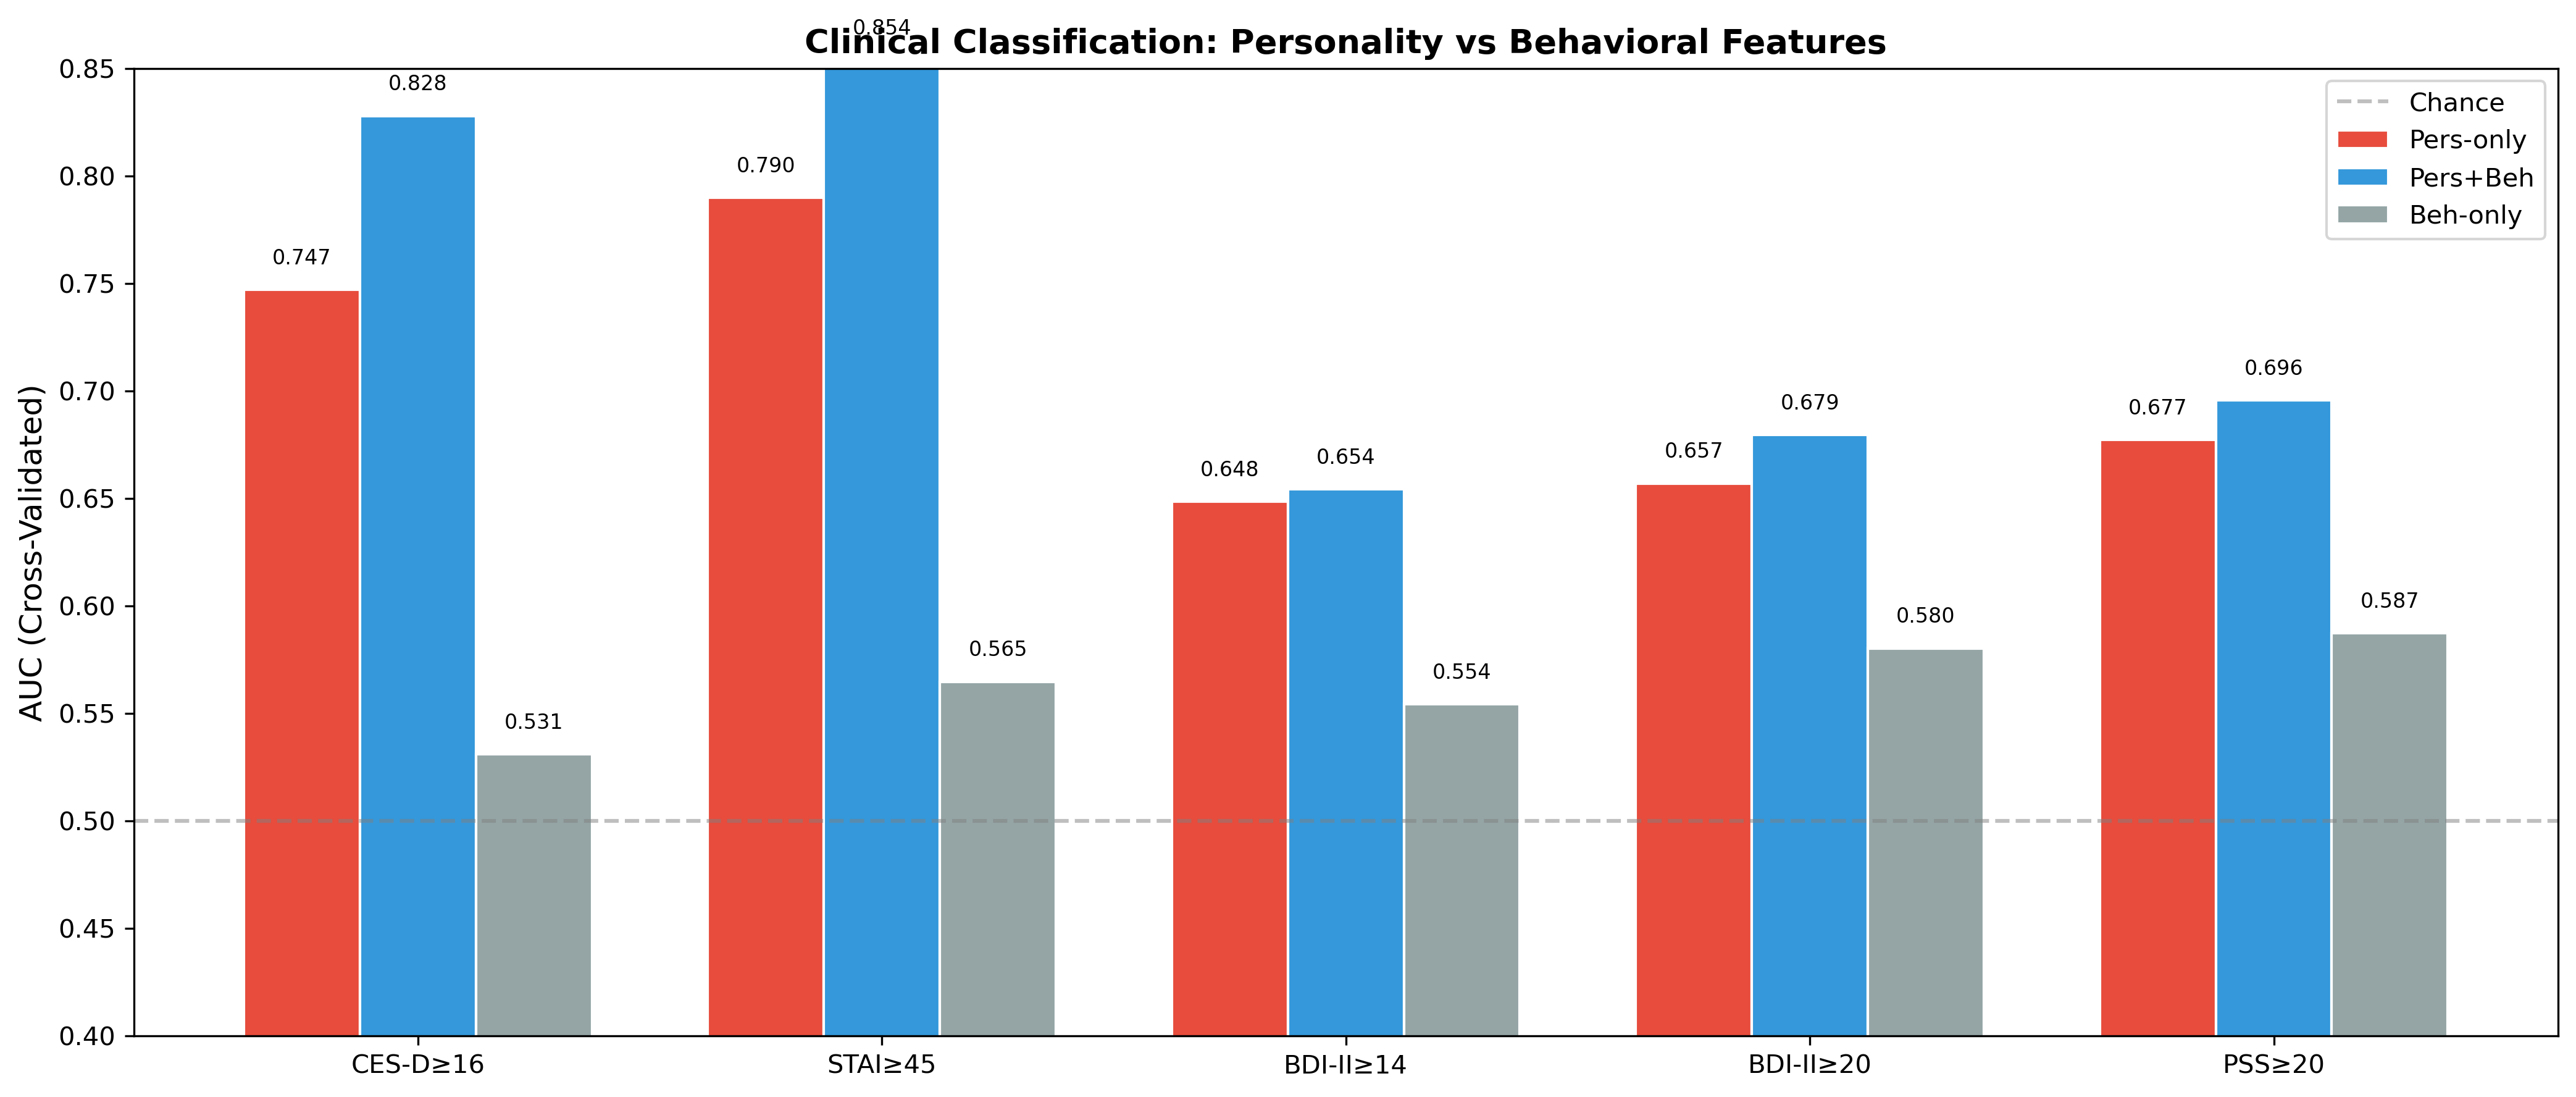
\includegraphics[width=\textwidth]{../results/comparison/figure18_clinical_classification.png}
\caption{Clinical classification performance (AUC) for personality-only, personality-plus-behavior, and behavior-only models across five classification targets in Studies 2 and 3. Error bars represent 95\% confidence intervals from repeated stratified 10$\times$10-fold cross-validation. Personality-only models consistently outperformed behavior-only models. Adding behavioral features provided modest but statistically non-significant improvement (DeLong $p_{\text{FDR}} > .44$ for all comparisons).}
\label{fig:clinical}
\end{figure}

\begin{figure}[htbp]
\centering
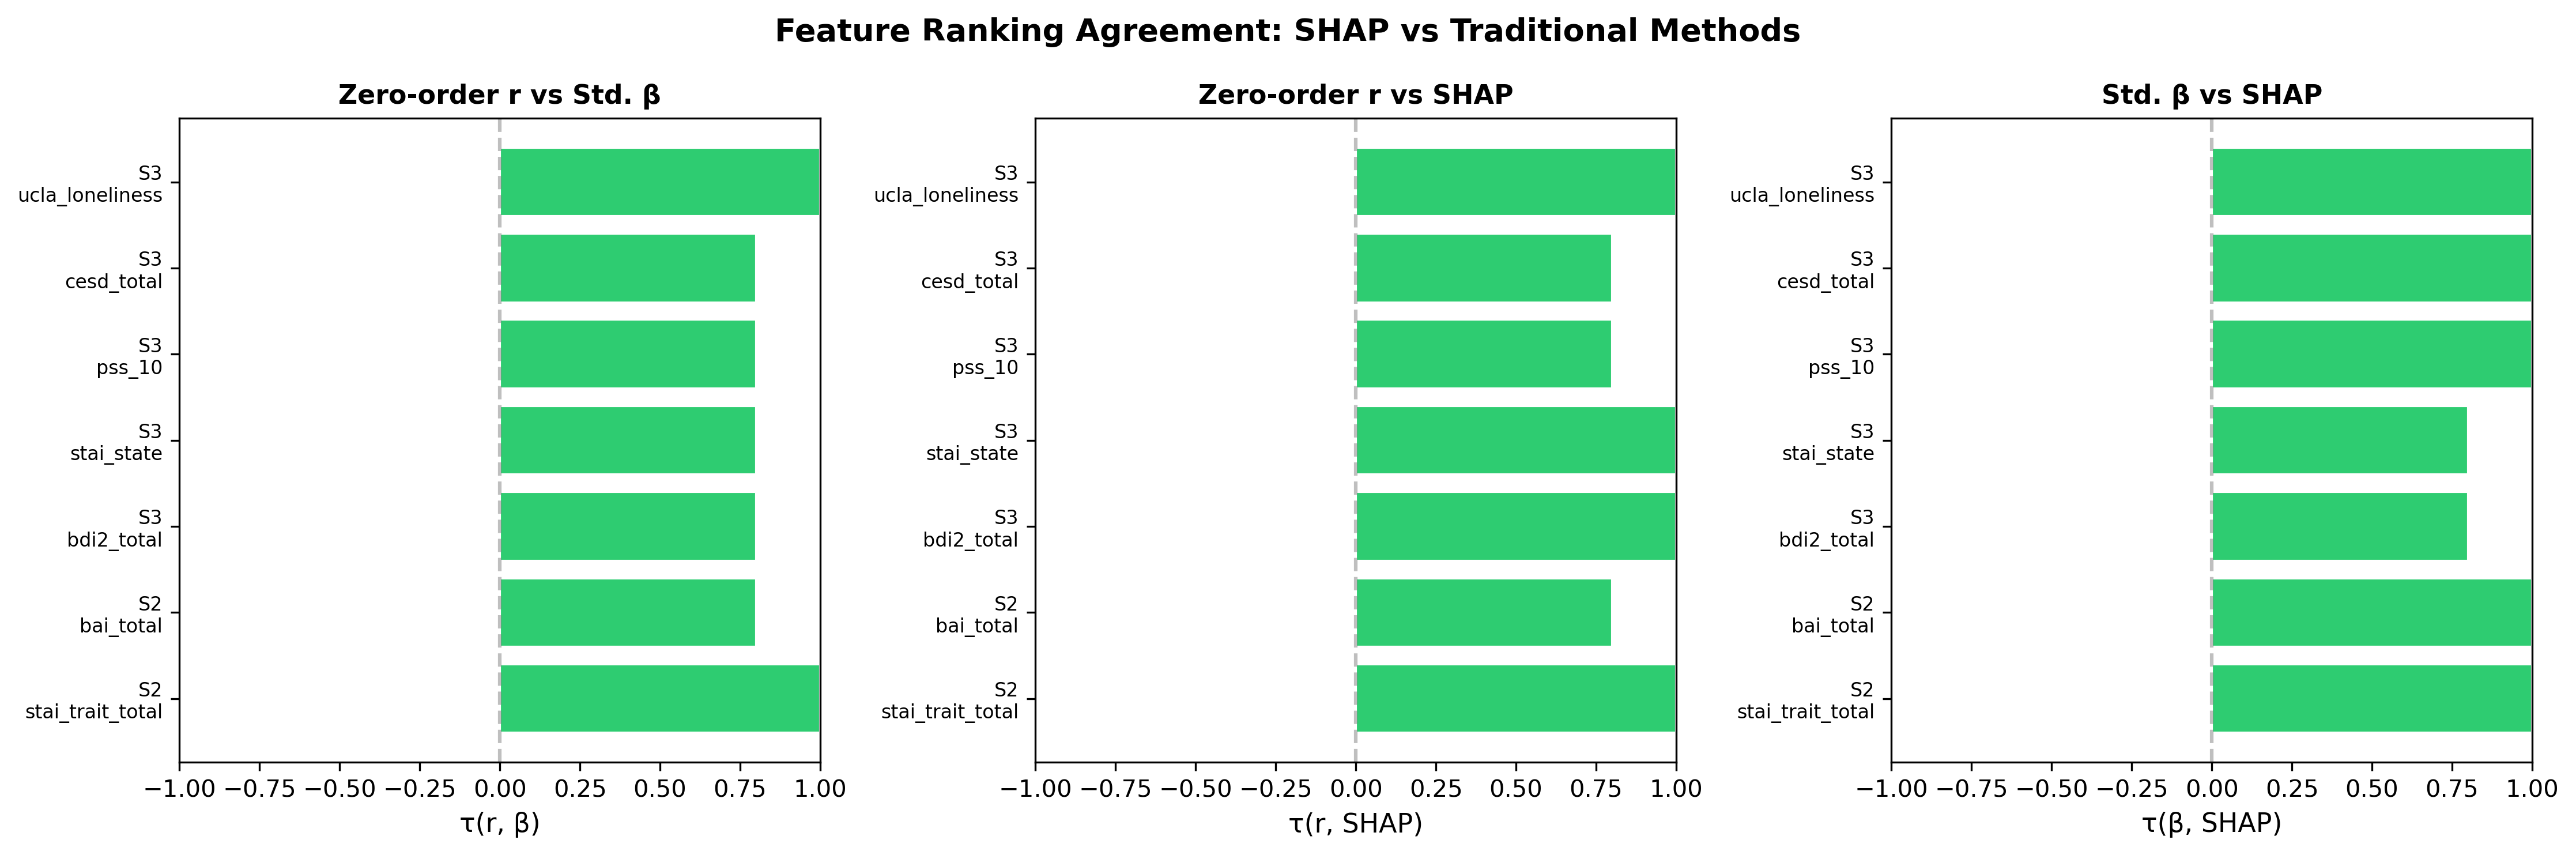
\includegraphics[width=\textwidth]{../results/comparison/figure19_shap_vs_traditional.png}
\caption{SHAP feature importance rankings compared with standardized OLS regression coefficients across seven outcomes in Studies 2 and 3. Kendall's $\tau$ between SHAP and OLS rankings averaged .94, indicating near-perfect agreement. Top-1 predictor agreement was 7/7 (100\%): Neuroticism for all mental health outcomes, Conscientiousness for GPA. This convergence suggests that machine learning interpretability methods confirm rather than extend traditional regression-based findings for personality--outcome associations.}
\label{fig:shap}
\end{figure}
